\section{Step 83 Delegate mandatory and fallback full records}
Fill \texttt{dr\_full\_call}. Reuse \texttt{video\_encode\_full} with the source address, exact source count, output address and shared context prefix. It admits its larger record count, emits a full record and commits the same sequence and previous-image fields. Return its status/count through the parent restore path. Its own validation remains part of its public contract, even though this caller has already validated source colors.

Use \texttt{s83-1} and stop before \texttt{dr\_full\_return}.

\paragraph{Observe} Use the sequence-zero recipe for \texttt{dr\_full\_return}. It produces a 12\,304-byte full record without reading old image contents or touching XOR scratch. The all-change and tie recipes reach the same branch after measuring candidate deltas.

Sequence zero must be independently decodable. Even though the supplied
\texttt{few} pair differs at only four pixels, this recipe requires a full record.
Its 12\,288 RGB payload bytes need the sixteen-byte header as well, producing
12\,304 bytes in total. Choosing the shorter delta at this boundary would change
the file's required starting state.

Inspect \texttt{delta\_output} plus three in the Memory tab's Bytes column.
The three leading \texttt{a5} guard bytes precede the record; they are not part of
its header. Kind zero and sequence zero are followed by payload length
\texttt{00 00 30 00}. The CRC is \texttt{1d 19 6e 30}, and the packed payload begins
\texttt{12 34 57}. Those three bytes represent the first numeric source word,
\texttt{0x00123457}. A little-endian native word would instead occupy memory as
\texttt{57 34 12 00}; the wire format still stores red, green and blue in that order.
Using the Bytes column keeps these two interpretations distinct.

To display the source picture, configure a custom Bitmap Display at
\texttt{delta\_source} plus four before launching Debug. Use 512 by 512 display
units, eight-unit pixels and \texttt{initial=true}. Here the source is initialized
in \texttt{.data} and remains read-only, so a write-only display would stay black.
The full encoder copies that source into the previous-image arena for a later call;
it does not need to form the candidate XOR image for this mandatory full record.

Figure~\ref{fig:video-record-selection} connects the source picture, record bytes,
shared context and return count. The context view shows kind zero and count
\texttt{0x3010}, with input pointers, capacity and the reserved pattern retained.
Also inspect context offset eight: its next sequence is now one. That field is
outside the cropped context detail. The parent is paused after its delegated call
and before \texttt{dr\_full\_return}'s \texttt{nop}.

% Native editable composition from verified, unchanged IDE images.
\begin{figure}[htbp]
  \centering
  \sbox0{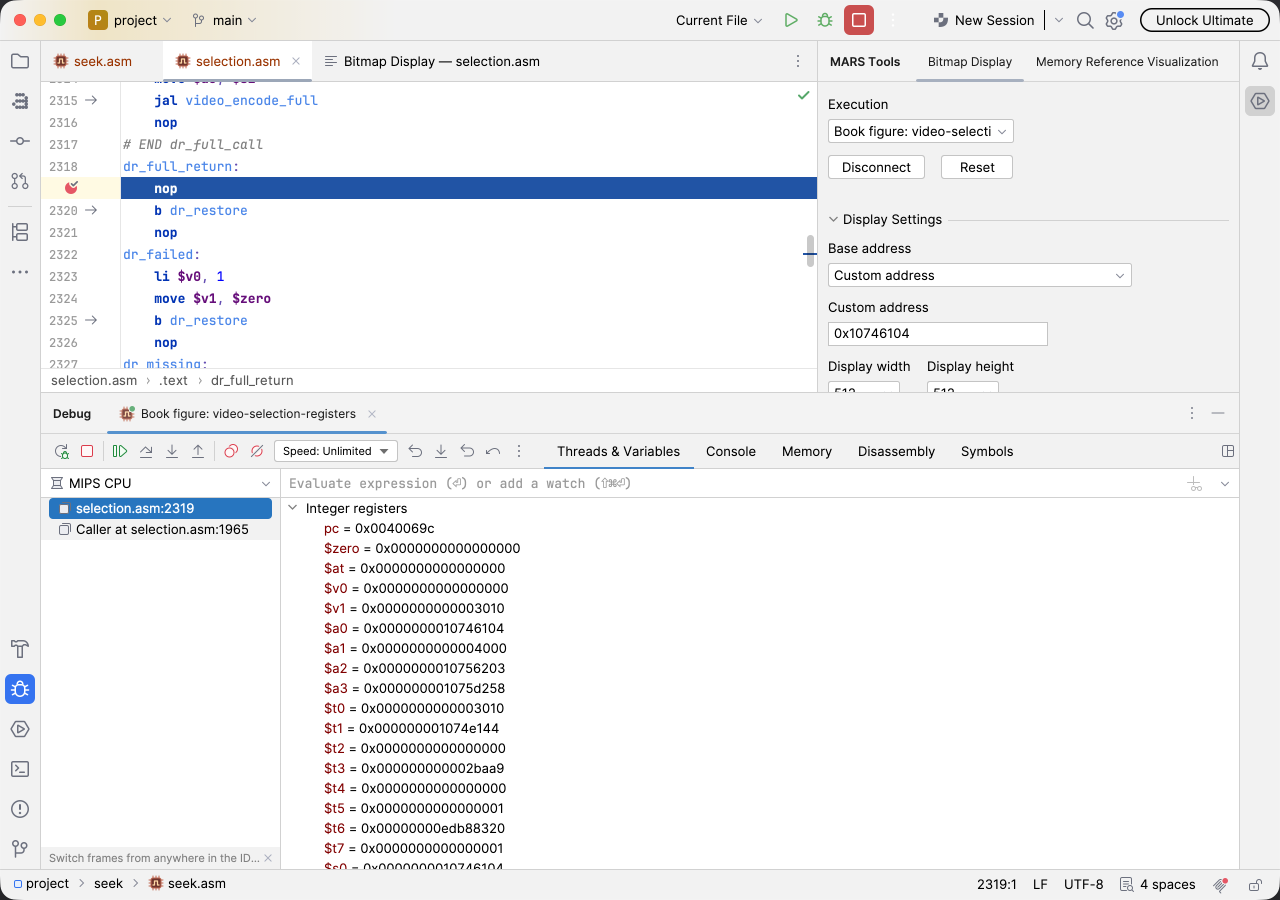
\includegraphics[artifact]{packages/034-lossless-video/captures/video-record-selection/registers.png}}
  \sbox2{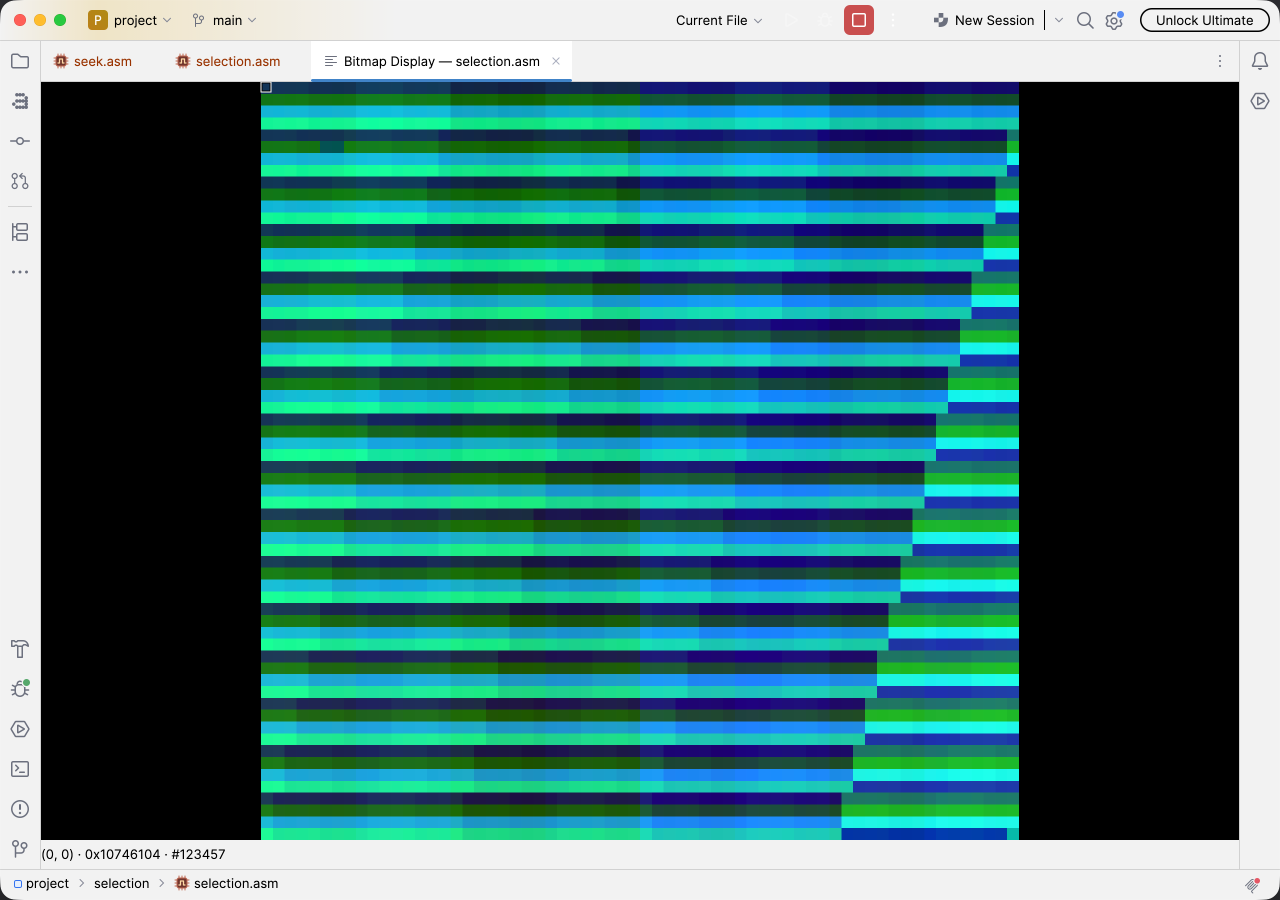
\includegraphics[artifact]{packages/034-lossless-video/captures/video-record-selection/bitmap.png}}
  \sbox4{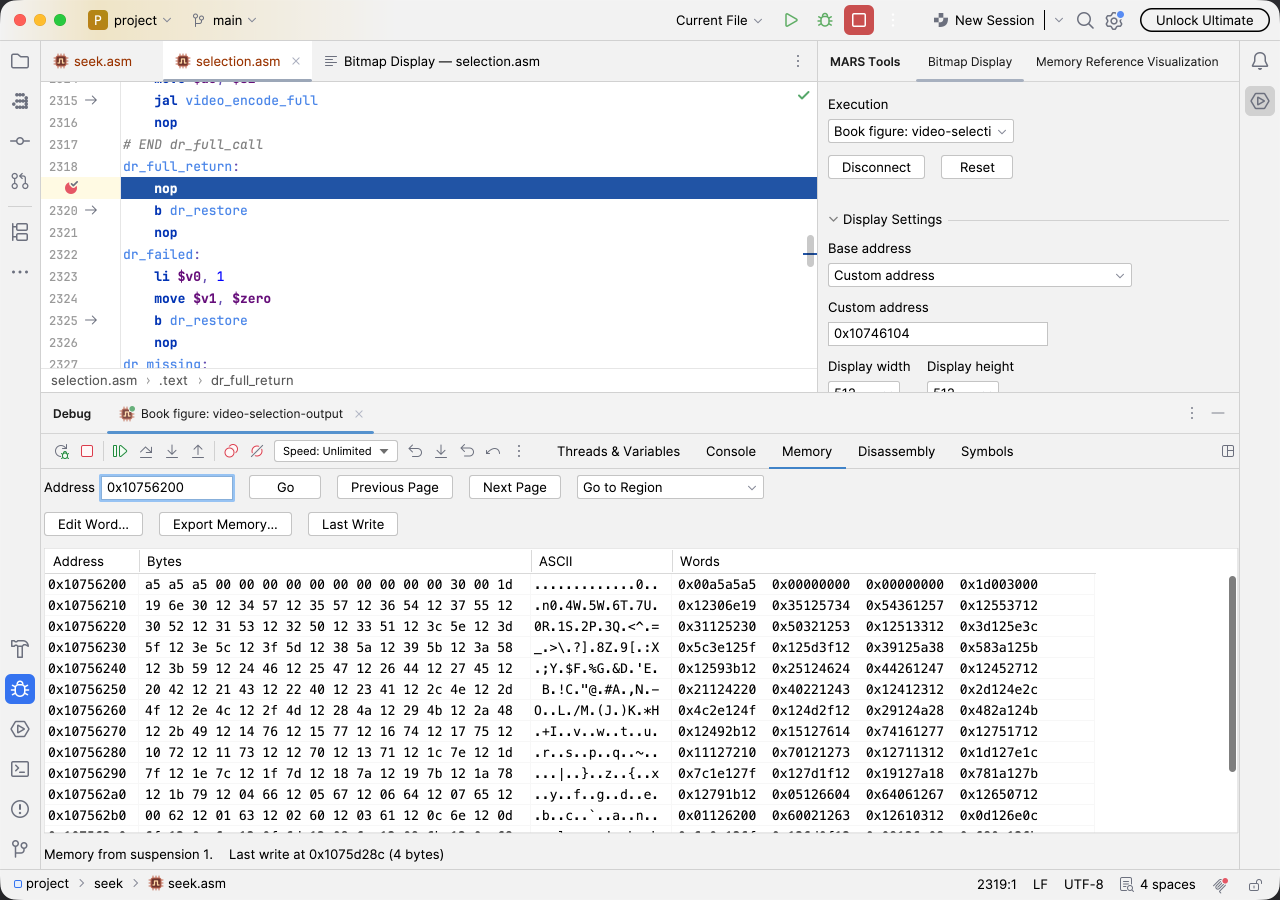
\includegraphics[artifact]{packages/034-lossless-video/captures/video-record-selection/output.png}}
  \sbox6{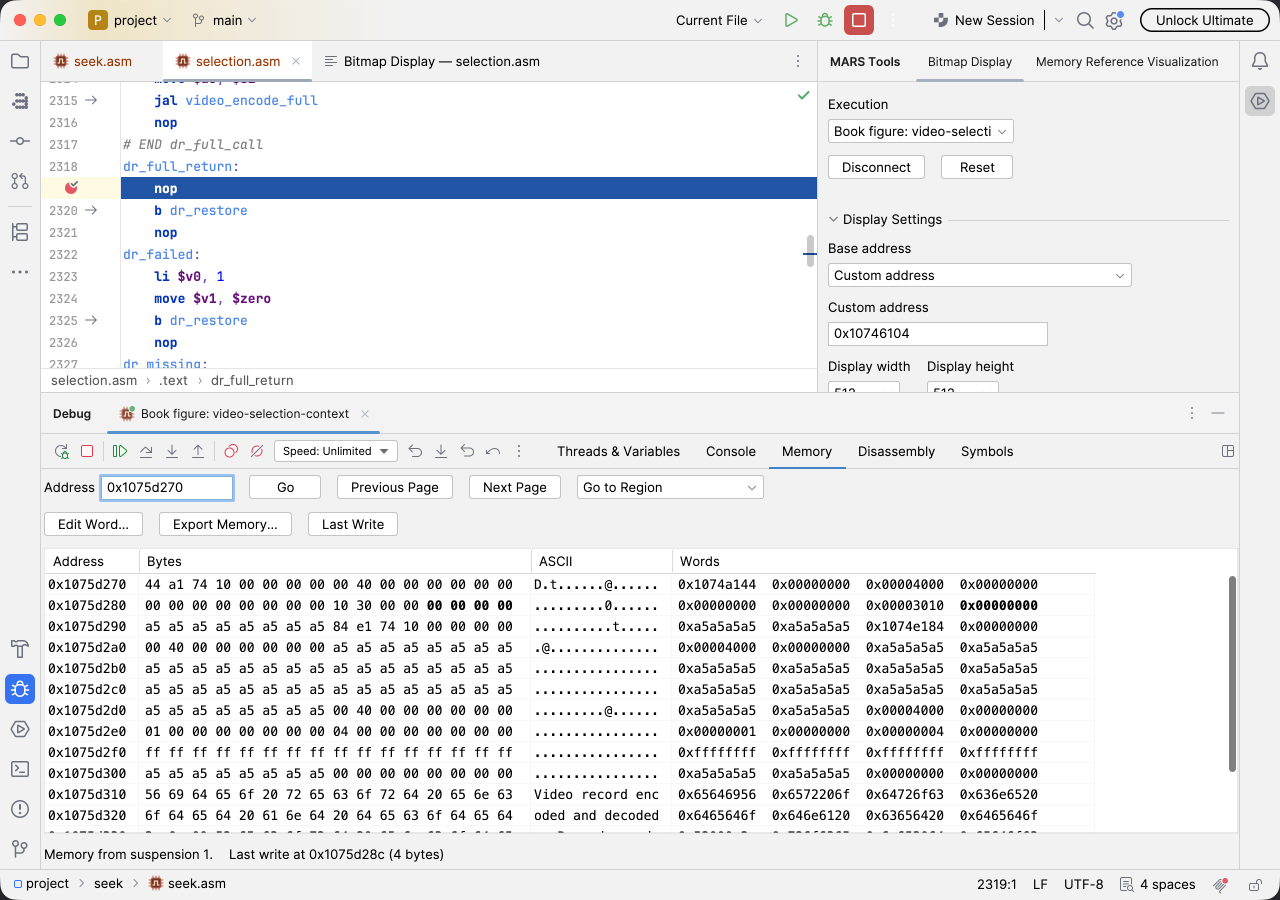
\includegraphics[artifact]{packages/034-lossless-video/captures/video-record-selection/context.png}}
  \edef\MARSselectionsourceLeft{\the\dimexpr0.036718750\wd0\relax}
  \edef\MARSselectionsourceBottom{\the\dimexpr0.774444444\ht0\relax}
  \edef\MARSselectionsourceRight{\the\dimexpr0.611718750\wd0\relax}
  \edef\MARSselectionsourceTop{\the\dimexpr0.170000000\ht0\relax}
  \edef\MARSselectionbitmapLeft{\the\dimexpr0.199218750\wd2\relax}
  \edef\MARSselectionbitmapBottom{\the\dimexpr0.060000000\ht2\relax}
  \edef\MARSselectionbitmapRight{\the\dimexpr0.199218750\wd2\relax}
  \edef\MARSselectionbitmapTop{\the\dimexpr0.084444444\ht2\relax}
  \edef\MARSselectionoutputLeft{\the\dimexpr0.108593750\wd4\relax}
  \edef\MARSselectionoutputBottom{\the\dimexpr0.288888889\ht4\relax}
  \edef\MARSselectionoutputRight{\the\dimexpr0.585156250\wd4\relax}
  \edef\MARSselectionoutputTop{\the\dimexpr0.634444444\ht4\relax}
  \edef\MARSselectioncontextLeft{\the\dimexpr0.520312500\wd6\relax}
  \edef\MARSselectioncontextBottom{\the\dimexpr0.288888889\ht6\relax}
  \edef\MARSselectioncontextRight{\the\dimexpr0.139843750\wd6\relax}
  \edef\MARSselectioncontextTop{\the\dimexpr0.634444444\ht6\relax}
  \edef\MARSselectionreturnsLeft{\the\dimexpr0.246093750\wd0\relax}
  \edef\MARSselectionreturnsBottom{\the\dimexpr0.310000000\ht0\relax}
  \edef\MARSselectionreturnsRight{\the\dimexpr0.596875000\wd0\relax}
  \edef\MARSselectionreturnsTop{\the\dimexpr0.638888889\ht0\relax}
  \begin{tikzpicture}[alt={Five annotated IDE details at dr_full_return. Detail 1 marks the next instruction after the full encoder returns. Detail 2 shows the source picture as a dark colored grid. Detail 3 shows the unaligned output bytes: three leading A5 guard bytes, kind zero, reserved zero bytes, sequence zero, payload length 0x3000, CRC 0x1d196e30, then RGB triples beginning 12 34 57 and 12 35 57. Detail 4 shows retained previous-image pointer and capacity, published kind zero and count 0x3010, retained A5 reserved field and scratch pointer. Detail 5 shows success v0 zero and v1 12304 record bytes.}]
    \node[anchor=north west,inner sep=0,font=\small\bfseries] (source-title) at (6mm,0) {Return from the shared full encoder};
    \node[anchor=north west,inner sep=0] (source) at ([yshift=-1mm]source-title.south west) {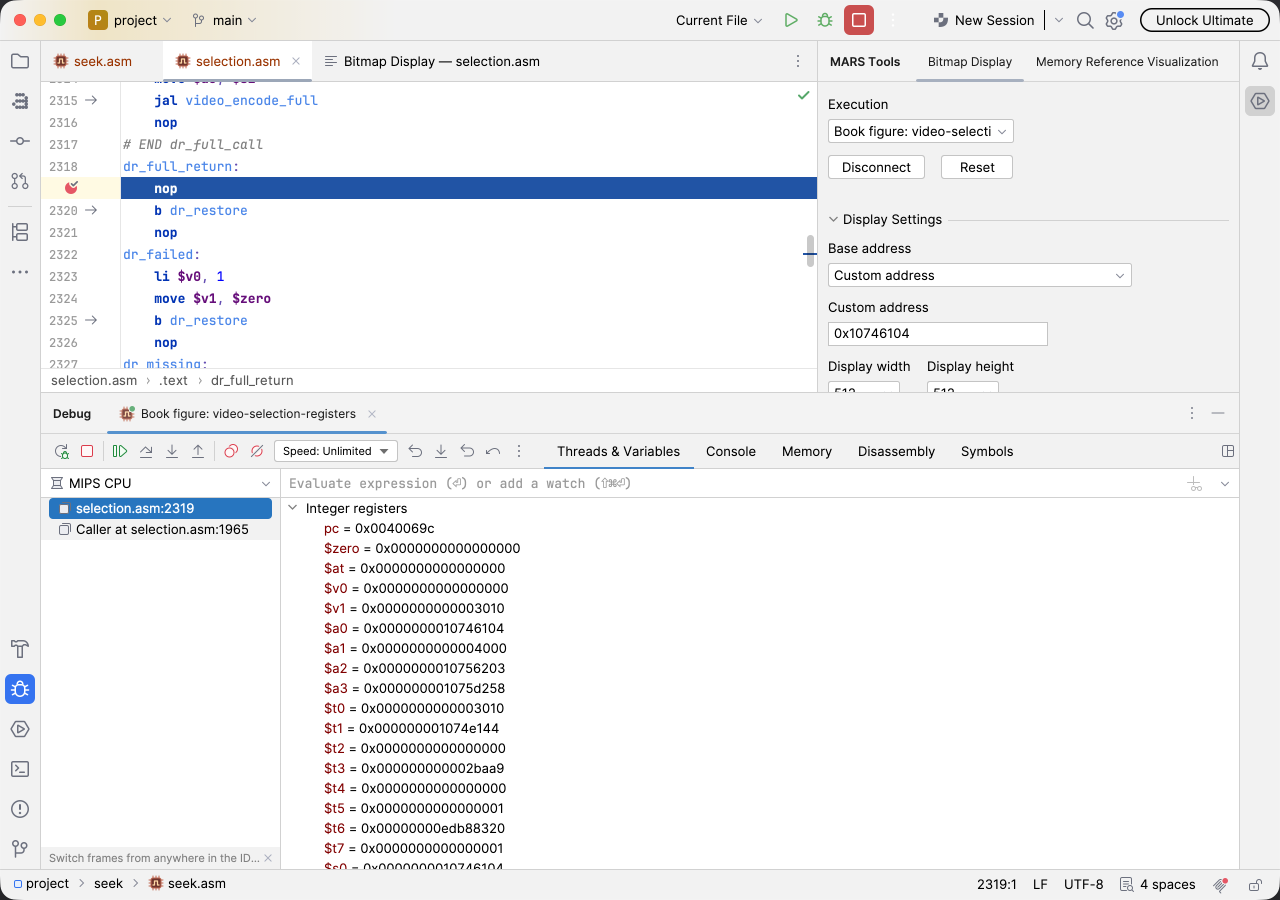
\includegraphics[width=0.64\linewidth,artifact,trim={\MARSselectionsourceLeft{} \MARSselectionsourceBottom{} \MARSselectionsourceRight{} \MARSselectionsourceTop{}},clip]{packages/034-lossless-video/captures/video-record-selection/registers.png}};
    \begin{scope}[shift={(source.south west)},x={($(source.south east)-(source.south west)$)},y={($(source.north west)-(source.south west)$)}]
      \draw[black,line width=0.7pt] (0.168888889,0.080000000) rectangle (0.288888889,0.520000000);
      \node[draw=black,fill=white,circle,inner sep=1.5pt,font=\footnotesize] at ($(0.168888889,0.520000000)+(-3mm,0)$) {1};
    \end{scope}
    \node[anchor=north west,inner sep=0,font=\small\bfseries] (bitmap-title) at ([yshift=-2mm]source.south west) {Read-only source picture};
    \node[anchor=north west,inner sep=0] (bitmap) at ([yshift=-1mm]bitmap-title.south west) {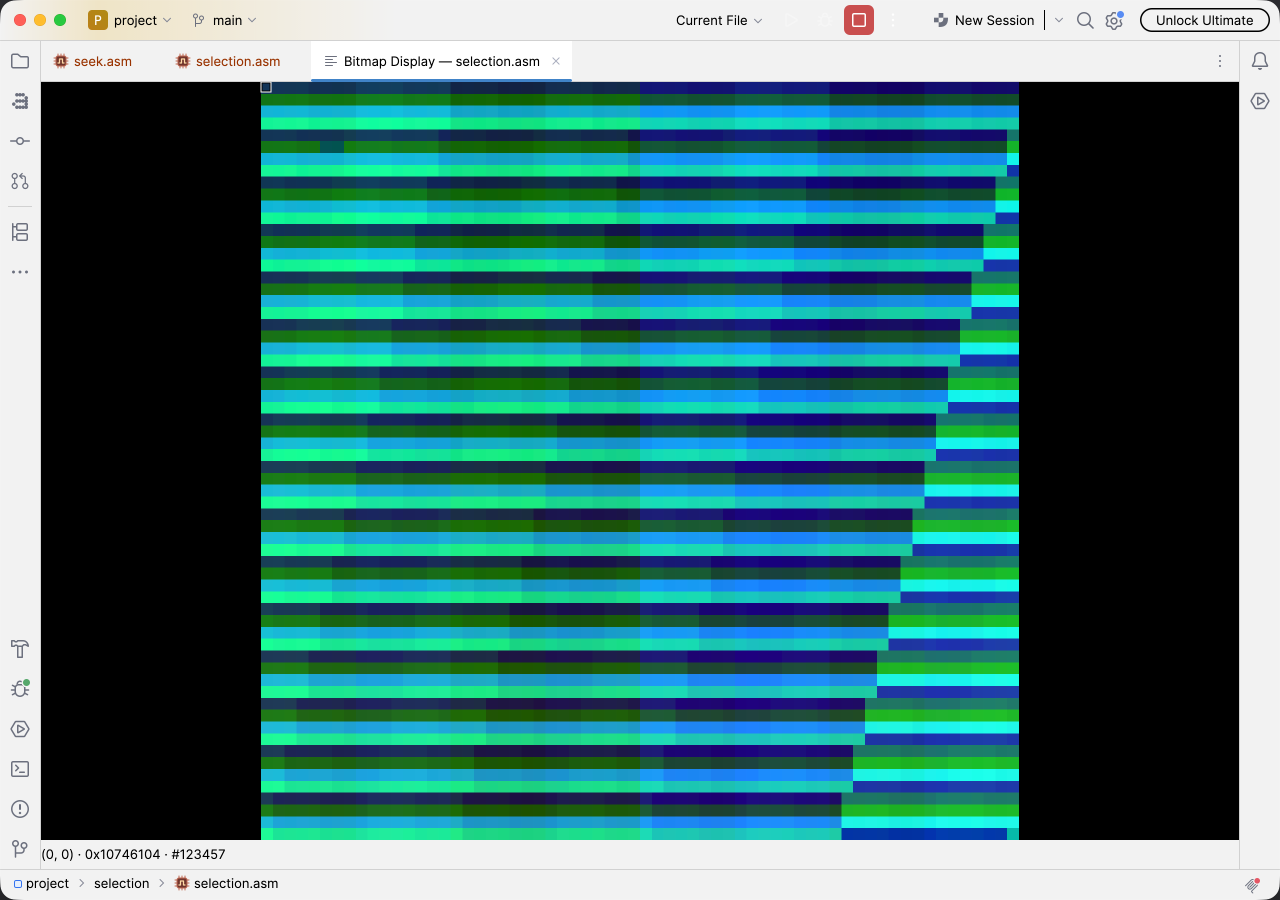
\includegraphics[width=0.24\linewidth,artifact,trim={\MARSselectionbitmapLeft{} \MARSselectionbitmapBottom{} \MARSselectionbitmapRight{} \MARSselectionbitmapTop{}},clip]{packages/034-lossless-video/captures/video-record-selection/bitmap.png}};
    \begin{scope}[shift={(bitmap.south west)},x={($(bitmap.south east)-(bitmap.south west)$)},y={($(bitmap.north west)-(bitmap.south west)$)}]
      \draw[black,line width=0.7pt] (0.007792208,0.007792208) rectangle (0.992207792,0.992207792);
      \node[draw=black,fill=white,circle,inner sep=1.5pt,font=\footnotesize] at ($(0.007792208,0.992207792)+(-3mm,0)$) {2};
    \end{scope}
    \node[anchor=north west,inner sep=0,font=\small\bfseries] (output-title) at ([yshift=-2mm]bitmap.south west) {Guard, full-record header and first RGB bytes};
    \node[anchor=north west,inner sep=0] (output) at ([yshift=-1mm]output-title.south west) {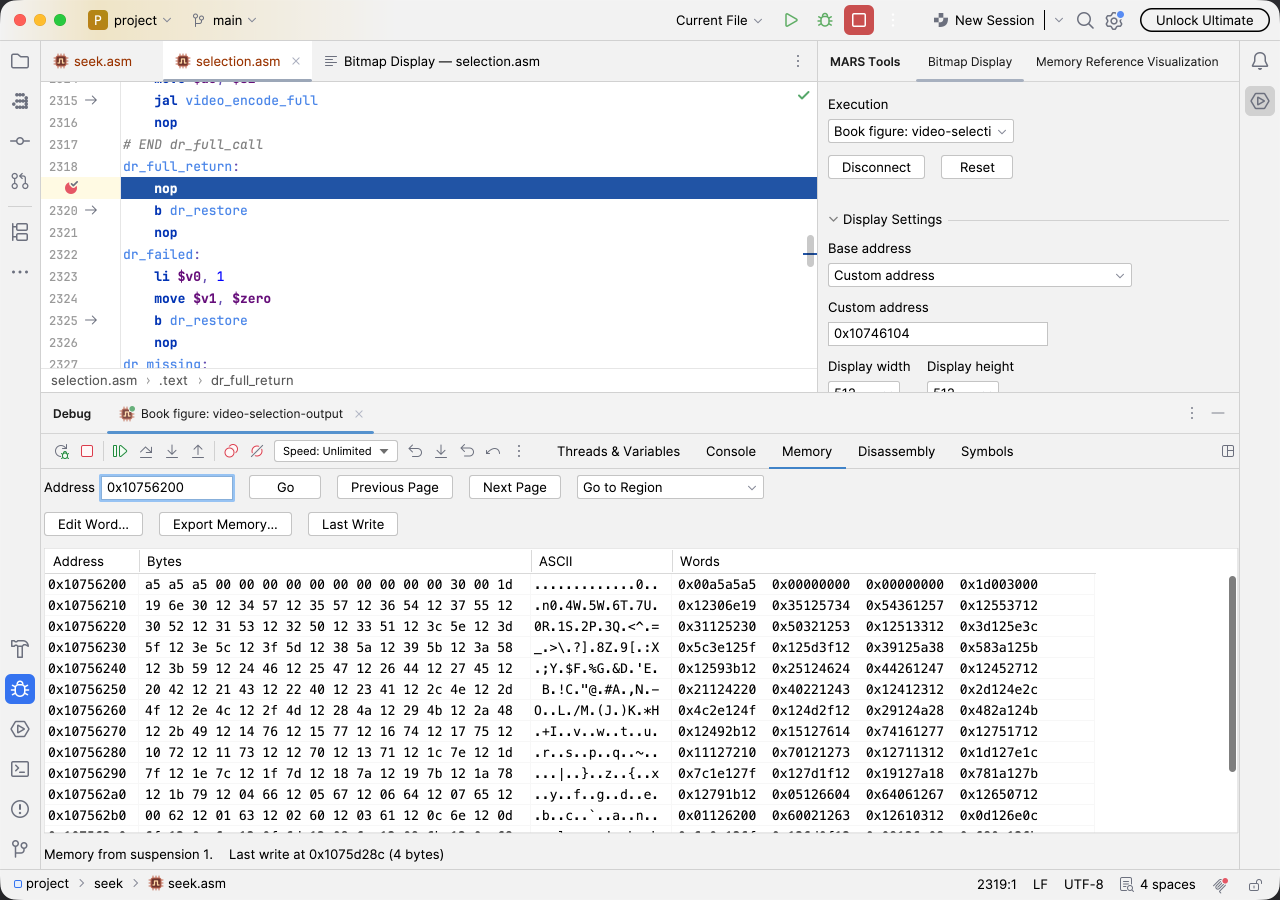
\includegraphics[width=0.83\linewidth,artifact,trim={\MARSselectionoutputLeft{} \MARSselectionoutputBottom{} \MARSselectionoutputRight{} \MARSselectionoutputTop{}},clip]{packages/034-lossless-video/captures/video-record-selection/output.png}};
    \begin{scope}[shift={(output.south west)},x={($(output.south east)-(output.south west)$)},y={($(output.north west)-(output.south west)$)}]
      \draw[black,line width=0.7pt] (0.000000000,0.043478261) rectangle (1.000000000,0.956521739);
      \node[draw=black,fill=white,circle,inner sep=1.5pt,font=\footnotesize] at ($(0.000000000,0.956521739)+(-3mm,0)$) {3};
    \end{scope}
    \node[anchor=north west,inner sep=0,font=\small\bfseries] (context-title) at ([yshift=-2mm]output.south west) {Shared-context publication and retained inputs};
    \node[anchor=north west,inner sep=0] (context) at ([yshift=-1mm]context-title.south west) {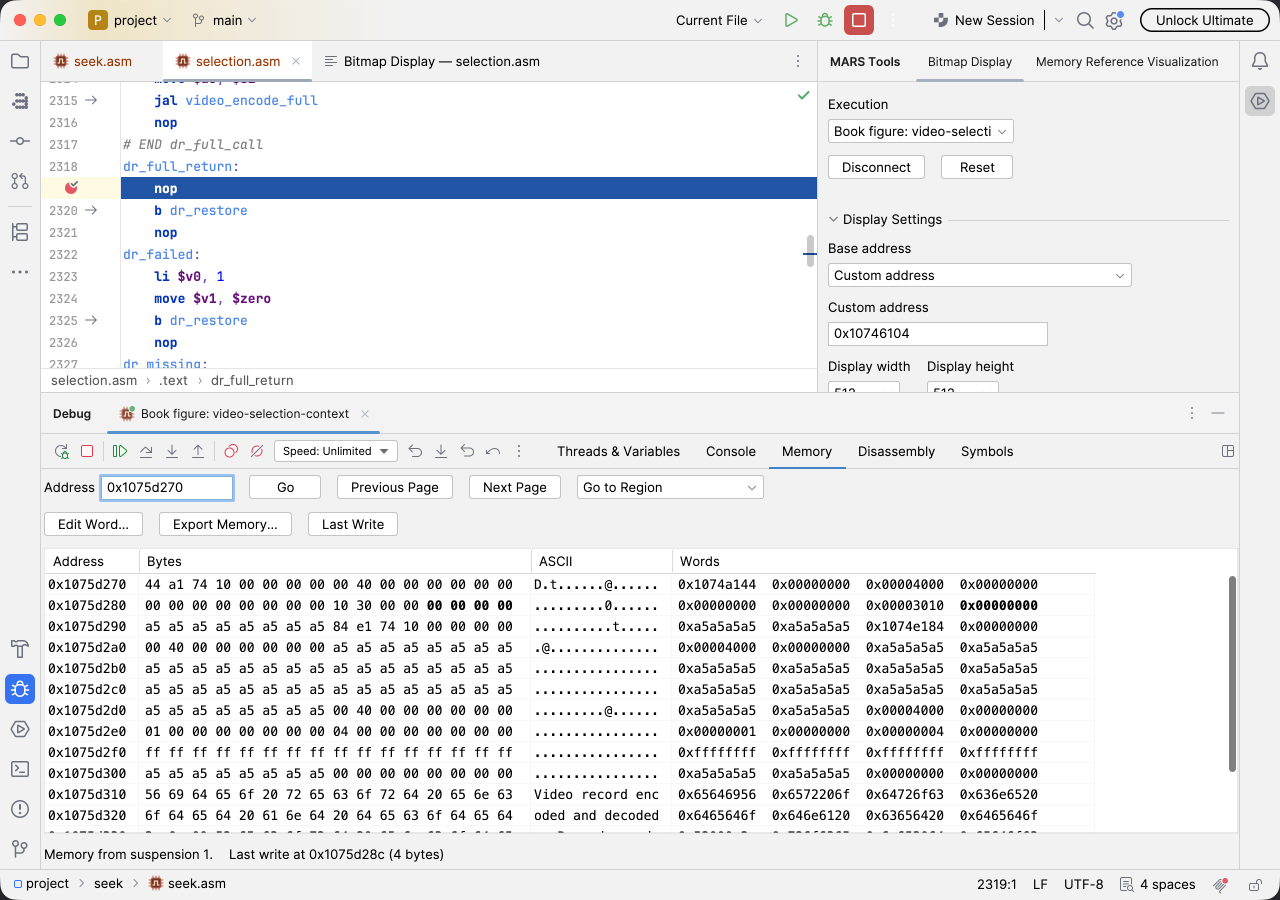
\includegraphics[width=0.74\linewidth,artifact,trim={\MARSselectioncontextLeft{} \MARSselectioncontextBottom{} \MARSselectioncontextRight{} \MARSselectioncontextTop{}},clip]{packages/034-lossless-video/captures/video-record-selection/context.png}};
    \begin{scope}[shift={(context.south west)},x={($(context.south east)-(context.south west)$)},y={($(context.north west)-(context.south west)$)}]
      \draw[black,line width=0.7pt] (0.013793103,0.043478261) rectangle (0.986206897,0.956521739);
      \node[draw=black,fill=white,circle,inner sep=1.5pt,font=\footnotesize] at ($(0.013793103,0.956521739)+(-3mm,0)$) {4};
    \end{scope}
    \node[anchor=north west,inner sep=0,font=\small\bfseries] (returns-title) at ([yshift=-2mm]context.south west) {Success and complete record size};
    \node[anchor=north west,inner sep=0] (returns) at ([yshift=-1mm]returns-title.south west) {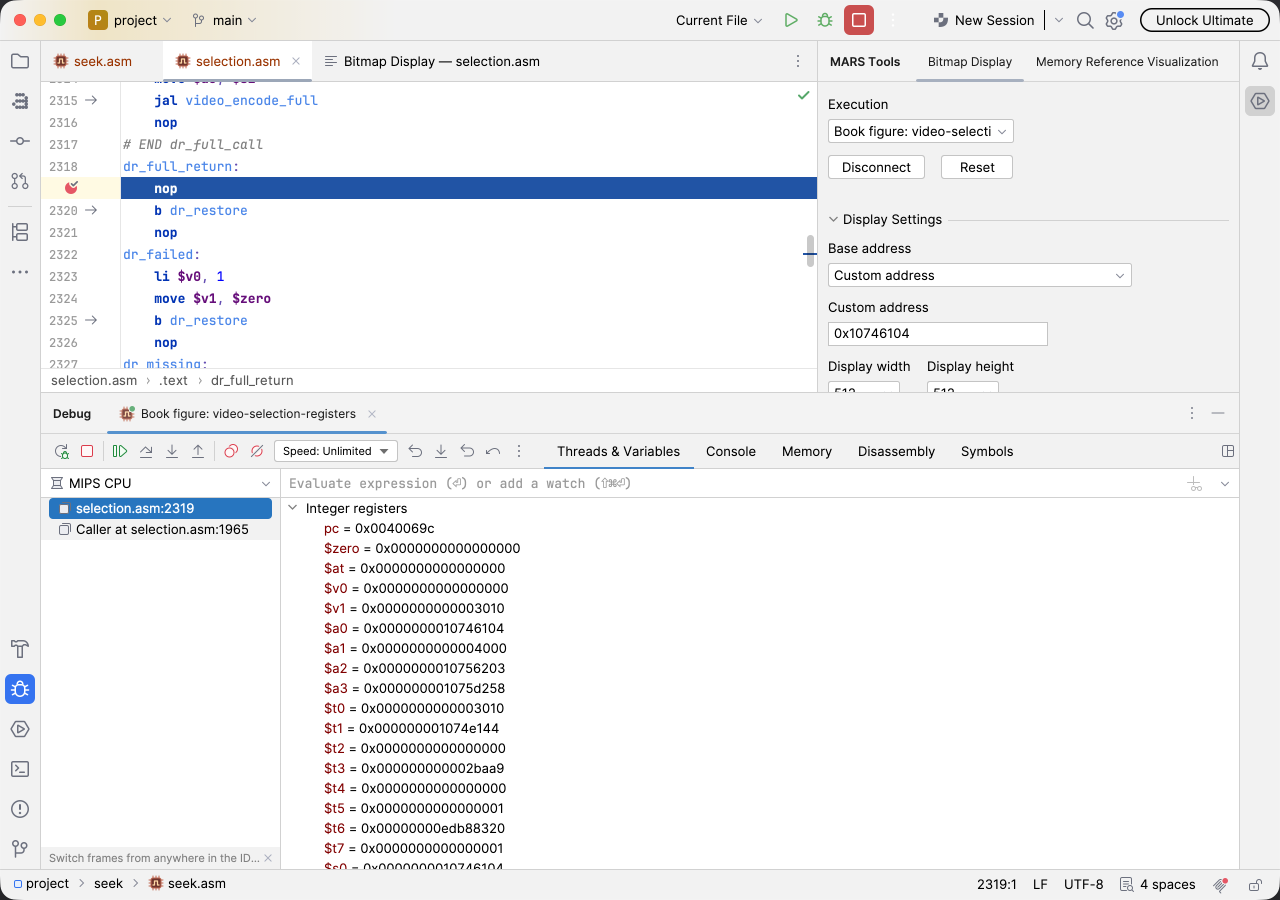
\includegraphics[width=0.48\linewidth,artifact,trim={\MARSselectionreturnsLeft{} \MARSselectionreturnsBottom{} \MARSselectionreturnsRight{} \MARSselectionreturnsTop{}},clip]{packages/034-lossless-video/captures/video-record-selection/registers.png}};
    \begin{scope}[shift={(returns.south west)},x={($(returns.south east)-(returns.south west)$)},y={($(returns.north west)-(returns.south west)$)}]
      \draw[black,line width=0.7pt] (0.029850746,0.065217391) rectangle (0.970149254,0.934782609);
      \node[draw=black,fill=white,circle,inner sep=1.5pt,font=\footnotesize] at ($(0.029850746,0.934782609)+(-3mm,0)$) {5};
    \end{scope}
  \end{tikzpicture}
  \par\smallskip
  \begin{minipage}{\linewidth}
    \small
    \begin{enumerate}
      \item The full encoder has returned; the parent checkpoint \texttt{nop} has not executed.
      \item The source picture remains unchanged. Its first numeric RGB word is \texttt{0x00123457}.
      \item Three leading \texttt{a5} bytes precede kind zero. The header carries sequence zero, payload length \texttt{0x3000} and CRC \texttt{0x1d196e30}. Packed RGB starts with \texttt{12 34 57}.
      \item Little-endian low/high pairs include the previous-image input, capacity \texttt{0x4000}, kind zero and count \texttt{0x3010}. The reserved \texttt{a5a5a5a5} field and scratch pointer are retained.
      \item \texttt{\$v0} is zero; \texttt{\$v1} is \texttt{0x3010}: 12\,288 payload bytes plus the sixteen-byte record header.
    \end{enumerate}
  \end{minipage}
  \caption{A mandatory full record at sequence zero. Four Debug launches inspect the same source, input and delegated-call return checkpoint.}
  \label{fig:video-record-selection}
\end{figure}

\clearpage

\Needspace{8\baselineskip}
\paragraph{Check} What does the shared full encoder update on success?
\begin{enumerate}[label=\Alph*.]
\item Only the CRC field.
\item The directory of an already opened video.
\item The same previous image and sequence/kind/count fields.
\end{enumerate}
